\boxde
\Opensolutionfile{ans}[ans/2D1-2-DEON-2]
\begin{ex}%[2D1B2-2]
    Cho hàm số $ f(x) $ có đạo hàm $ f'(x) = x(x-1)^4(x+2)^3 $. Số điểm cực trị của hàm số đã cho là
    \choice
    {$ 3 $}
    {\True $ 2 $}
    {$ 8 $}
    {$ 1 $}
    \loigiai{
        Ta có $ f'(x)=0 \Leftrightarrow \hoac{& x=0\\&x=1\\&x=-2} $. Trong đó các nghiệm bội lẻ là $ x=0 $ và $ x=-2 $. Do đó, hàm số đã cho có hai điểm cực trị.
    }
\end{ex}
\begin{ex}%[2D1K2-2]
    \immini{Cho hàm số $ y=f(x)$ có đồ thị hàm $ y=f'(x) $ như hình vẽ. Số điểm cực trị của hàm số đã cho là
        \choice[2]
        {$ 4 $}
        { $ 1 $}
        {\True$ 2 $}
        {$ 3 $}}{
        \begin{tikzpicture}[font=\footnotesize, line join=round, line cap=round, >=stealth, scale=0.5]
            \draw[->] (0,-2)--(0,3)node[right]{$y$};
            \draw[->] (-3,0)--(0,0)node[above right] {$ O $}--(3,0)node[below]{$x$};
            \draw (0,0) .. controls (0.5,-0.1) and (1.5,-3.5) .. (2,0)node[below right]{$ 2 $};
            \draw (-1,0)node[below left]{$ -1 $} .. controls (-0.7,-0.6) .. (0,0);
            \draw (-1,0) .. controls (-1.5,1.2) .. (-1.7,2);
            \draw (2,0) .. controls (2.1,1.5) .. (2.1,2)node[right]{$ f'(x) $};
        \end{tikzpicture}
    }
    \loigiai
    {
        Dựa vào đồ thị, ta lập bảng biến thiên
        \begin{center}
            
\begin{tikzpicture}[scale=.9, font=\footnotesize, line join=round, line cap=round, >=stealth]
                \tkzTabInit[nocadre=false,lgt=1,espcl=2,deltacl=0.5]{$x$/.7 ,$f'(x)$/.7,$f(x)$/2}
                {$-\infty$ , $-1$, $ 0 $ , $2$ , $+\infty$}
                \tkzTabLine{ , + , $0$ , - , $0$ , - ,$ 0 $,+ }
                \tkzTabVar{-/ , +/ , R ,-/, +/}
            \end{tikzpicture}
        \end{center}
        Từ bảng biến thiên ta thấy, đồ thị hàm số $ f(x) $ có hai điểm cực trị.
    }
\end{ex}
\begin{ex}%[2D1K2-2]
    Cho hàm số $y=f(x)$ liên tục trên $\mathbb{R}$ và hàm số $f'(x)$ có bảng biến thiên như sau. Tìm mệnh đề đúng.
    \begin{center}
        
\begin{tikzpicture}
            \tkzTabInit[nocadre=false,lgt=1.2,espcl=2.5,deltacl=0.6]
            {$x$ /0.6,$f''(x)$ /0.6,$f'(x)$ /2}
            {$-\infty$,$-1$,$1$,$+\infty$}
            \tkzTabLine{,+,$0$,-,$0$,+,}
            \tkzTabVar{-/$-\infty$, +/$2$,-/$-1$,+/$+\infty$}
        \end{tikzpicture}
    \end{center}
    \choice
    {\True Hàm số $y=f(x)$ có $2$ điểm cực tiểu và $1$ điểm cực đại}
    {Hàm số $y=f(x)$ có $1$ điểm cực tiểu và $1$ điểm cực đại}
    {Hàm số $y=f(x)$ không có giá trị lớn nhất và không có giá trị nhỏ nhất}
    {Hàm số $y=f(x)$ có $1$ điểm cực tiểu và $2$ điểm cực đại}
    \loigiai{
        Từ bảng biến thiên, ta thấy $f'(x)=0 \Leftrightarrow \hoac{& x=a<-1\\& x=b\in(-1;1)\\& x=c>1.}$\\
        Ta có bảng biến thiên của hàm số $y=f(x)$
        \begin{center}
            
\begin{tikzpicture}
                \tkzTabInit[nocadre=false,lgt=1.2,espcl=2.5,deltacl=0.6]
                {$x$ /0.6,$f'(x)$ /0.6,$f(x)$ /2}
                {$-\infty$,$a$,$b$,$c$,$+\infty$}
                \tkzTabLine{,-,$0$,+,$0$,-,$0$,+,}
                \tkzTabVar{+/,-/,+/,-/,+/}
            \end{tikzpicture}
        \end{center}
        Do đó mệnh đề đúng là ``Hàm số $y=f(x)$ có $2$ điểm cực tiểu và $1$ điểm cực đại''.
    }
\end{ex}

%D:\Khanh\Toan Ly Hoa\Toan\BTTEXPRO\OUTPUT\Question Bank\[2D1K2-2].tex
\begin{ex}%[2D1K2-2]
    Cho hàm số $ y=f(x)$, biết $f'(x)$ có đồ thị như hình bên dưới.
    \begin{center}
        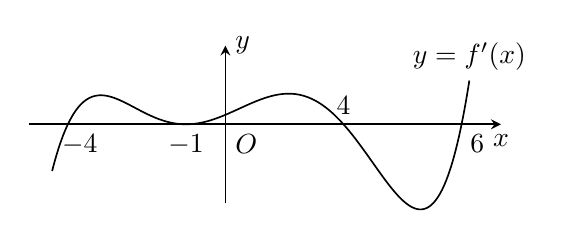
\begin{tikzpicture}[>=stealth,samples=100,smooth,color=black,line width=0.6pt]
            \begin{scope}[scale=.5]
                \draw[->] (-5,0)--(7,0) node[below] {$x$};
                \draw[->] (0,-2)--(0,2) node[right] {$y$};
                \draw (0,0) node [below right] {$O$};
                \draw[samples=200,domain=-4.4:6.2,smooth,variable=\x]
                plot (\x,{((\x)+4)*((\x)+1)^2*((\x)-3)*((\x)-6)/300})node[above]{$y=f'(x)$};
                \path
                (3,0)node[above]{$4$}
                (-1,0)node[below]{$-1$}
                (6,0)node[below,xshift=0.2cm]{$6$}
                (-4,0)node[below,xshift=0.15cm]{$-4$}
                ;
            \end{scope}
        \end{tikzpicture}
    \end{center}
    Khằng định nào sau đây \textbf{sai} ?
    \choice
    {Hàm số $ f(x)$ đạt cực đại tại điểm $ x=4$}
    {Hàm số $ f(x)$ đạt cực tiểu tại các điểm $ x=-4$ và $ x=6$}
    {\True Hàm số $ f(x)$ có 4 điểm cực trị}
    {Hàm số $ f(x)$ có 3 điểm cực trị}
    \loigiai{
        Dựa vào đồ thị của $y=f'(x)$ ta có bảng biến thiên
        \begin{center}
            
\begin{tikzpicture}
                \tkzTabInit[lgt=1.2,espcl=2.5]
                {$x$/0.7,$f’(x)$/0.7,$f(x)$/2.5}
                {$-\infty$,$-4$,$-1$,$4$,$6$,$+\infty$}
                \tkzTabLine{,-,0,+,0,+,0,-,0,+,}
                \tkzTabVar{+/,-/,R,+/,-/,+/}
            \end{tikzpicture}
        \end{center}
        Hàm số có $3$ điểm cực trị.
}\end{ex}
\begin{ex}%[2D1K2-2]
    \immini{
        Cho hàm số $y=f(x)$ có đạo hàm liên tục trên $\mathbb R$, đồ thị của hàm số $y=f'(x)$ là đường cong ở hình bên. Mệnh đề nào sau đây đúng?
        \choice
        {Hàm số $y=f(x)$ đạt cực đại tại $x=3$}
        {Hàm số $y=f(x)$ có một điểm cực tiểu thuộc khoảng $(2;3)$}
        {Hàm số $y=f(x)$ có đúng $2$ điểm cực trị}
        {\True Hàm số $y=f(x)$ đạt cực tiểu tại $x=3$}
    }
    {
        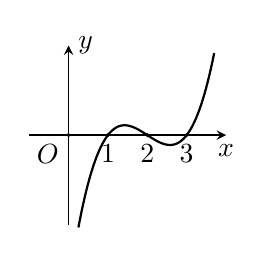
\begin{tikzpicture}[>=stealth,x=1cm,y=0.65cm,scale=0.5]
            \draw[->,line width = 0.5pt] (-1,0)--(4,0) node[below]{$x$};
            \draw[->,line width = 0.5pt] (0,-3.5) --(0,3.5) node[right]{$y$};
            \draw (0,0) node[below left]{$O$} [fill=black] circle (1pt);
            \draw (2,0) node[below]{$2$} [fill=black] circle (1pt);
            \draw (1,0) node[below]{$1$} [fill=black] circle (1pt);
            \draw (3,0) node[below]{$3$} [fill=black] circle (1pt);
            \draw [thick,samples=100, domain=0.25:3.7] plot (\x, {(\x-1)*(\x-2)*(\x-3)});
        \end{tikzpicture}
    }
    \loigiai{
        Từ đồ thị hàm số $y=f'(x)$ ta có bảng biến thiên của hàm số $y=f(x)$.
        \begin{center}
            
\begin{tikzpicture}
                \tkzTabInit[lgt=1.5,espcl=2.5,deltacl=.5]
                {$x$ /.7, $f'(x)$ /.7,$f(x)$ /2}
                {$-\infty$ , $1$ , $2$ , $3$ , $+\infty$}
                \tkzTabLine{ ,-,0,+,0,-,0,+, }
                \tkzTabVar{+/$+\infty$ ,-/ $f(1)$ ,+/$f(2)$, -/$f(3)$,+/$+\infty$}
            \end{tikzpicture}
        \end{center}
        Dựa vào bảng biến thiên ta có hàm số $y=f(x)$ đạt cực tiểu tại $x=3$.
    }
\end{ex}
\begin{ex}%[2D1B2-2]
    Cho hàm số $y=f(x)$ có bảng xét dấu của đạo hàm như hình vẽ.
    \begin{center}
        
\begin{tikzpicture}
            \tkzTabInit[espcl=2.5,lgt=1]
            {$x$/0.7,$y'$/0.7}
            {$-\infty$,$-2$,$1$,$3$,$+\infty$}
            \tkzTabLine{,-,0,+,0,+,0,-}
        \end{tikzpicture}
    \end{center}
    Hàm số $y=f(x)$ có bao nhiêu điểm
    cực đại?
    \choice
    {$ 2  $}
    {\True $ 1  $}
    {$ 3  $}
    {$ 0 $}
    \loigiai{
        \begin{center}
            
\begin{tikzpicture}
                \tkzTabInit[espcl=2.5,lgt=1.5]
                {$x$/0.7,$y'$/0.7,$y$/2.2}
                {$-\infty$,$-2$,$1$,$3$,$+\infty$}
                \tkzTabLine{,-,z,+,z,+,z,-}
                \tkzTabVar{+/,-/,R/,+/,-/}
            \end{tikzpicture}
        \end{center}
        Hàm số có một điểm cực đại.
    }
\end{ex}
\begin{ex}%[2D1B2-2]
    Cho hàm số $ f(x) $ có đạo hàm $ f'(x)=x(x-1)(x+2)^3 $, $ \forall x \in \mathbb{R} $. Số điểm cực trị của hàm số đã cho là
    \choice
    {\True $ 3 $}
    {$ 2 $}
    {$ 5 $}
    {$ 1 $}
    \loigiai{
        Ta có $ f'(x)=0 \Leftrightarrow \hoac{&x=0\\&x=1\\&x=-2} $. Ba nghiệm này đều là nghiệm bội lẻ nên hàm số đã cho có ba điểm cực trị.
    }
\end{ex}
\begin{ex}%[2D1B2-1]
    Cho hàm số $y=f(x)$ liên tục trên $\mathbb{R}$, có đạo hàm $f'(x)=x^3\left(x-1\right)^2\left(x+2\right)$. Hỏi hàm số $ y=f(x)$ có bao nhiêu điểm cực trị?
    \choice
    {\True $ 2$}
    {$ 0$}
    {$ 1$}
    {$ 3$}
    \loigiai
    {
        Hàm số $y=f(x)$ có đạo hàm trên $\mathbb{R}$ và $f'(x)=0\Leftrightarrow\hoac{&
            x=0\\&
            x=1\\&
            x=-2}$, trong đó $x=1$ là nghiệm kép.\\
        Vậy hàm số $y=f(x)$ có $2$ điểm cực trị.
    }
\end{ex}
\begin{ex}%[2D1K2-1]
    Đồ thị hàm số $y=x^3+x^2-5x+1$ có hai điểm cực trị $A$ và $B$. Điểm nào dưới đây là trung điểm của đoạn thẳng $AB$ ?
    \choice
    {\True $M\left( -\dfrac{1}{3};\dfrac{74}{27}\right)$}
    {$N\left( -\dfrac{2}{3};\dfrac{148}{27}\right)$}
    {$P\left( \dfrac{8}{3};\dfrac{256}{27}\right)$}
    {$Q\left( \dfrac{4}{3};\dfrac{128}{27}\right)$}
    \loigiai{
        Ta có $y'=3x^2+2x-5$ luôn có hai nghiệm phân biệt nên đồ thị hàm số $y=x^3+x^2-5x+1$ luôn có hai điểm cực trị $A$ và $B$.\\
        Do $y=x^3+x^2-5x+1$ là hàm bậc ba nên điểm uốn $U$ chính là trung điểm của $AB$.\\
        Ta có $y''=6x+2$; $y''=0 \Leftrightarrow 6x+2=0 \Leftrightarrow x = -\dfrac{1}{3}$.\\
        Vậy tọa độ điểm uốn là $U\left( -\dfrac{1}{3};\dfrac{74}{27}\right)$.
    }
\end{ex}
\begin{ex}%[2D1B2-1]
    Tìm tọa độ điểm cực đại của đồ thị hàm số $y=2x^3-3x^2+5$.
    \choice
    {$(1; 4)$}
    {\True $(0; 5)$}
    {$(5; 0)$}
    {$(4; 1)$}
    \loigiai{
        Hàm bậc ba có $y'=0\Leftrightarrow 6x^2-6x=0\Leftrightarrow\hoac{&x=0\\&x=1.}$\\
        Bảng biến thiên của hàm số
        \begin{center}
            
\begin{tikzpicture}
                \tkzTabInit[nocadre=false,lgt=1.2,espcl=2.5,deltacl=0.6]
                {$x$ /0.6,$y'$ /0.6,$y$ /2}
                {$-\infty$,$0$,$1$,$+\infty$}
                \tkzTabLine{,+,$0$,-,$0$,+,}
                \tkzTabVar{-/$-\infty$,+/$5$,-/$4$,+/$+\infty$}
            \end{tikzpicture}
        \end{center}
        Vậy tọa độ điểm cực đại của đồ thị hàm số là $(0; 5)$.
    }
\end{ex}
%%câu 7
\begin{ex}%[2D1Y2-2]
    Cho hàm số $y= f(x)$ có bảng biến thiên như sau
    \begin{center}
        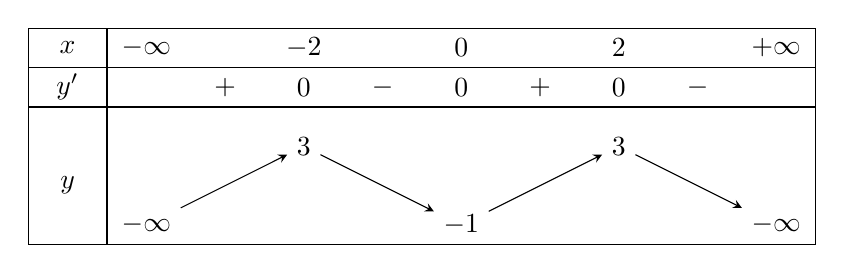
\begin{tikzpicture}[yscale=.5,xscale=1,
            kxd/.pic={\draw[double] (90:.5)--(-90:.5);}]
            \begin{scope}[shift={(-.5,.5)}]
                \draw
                (0,0) rectangle +(10,-5.5)
                (0,-1)--+(0:10) (0,-2)--+(0:10) (1,0)--+(-90:5.5);
            \end{scope}
            \path
            (0,0) node{$x$} % <<< dòng 1
            ++(0:1) node{$-\infty$}
            ++(0:2) node{$-2$}
            ++(0:2) node{$0$}
            ++(0:2) node{$2$}
            ++(0:2) node{$+\infty$}
            (0,-1) node{$y'$} % <<< dòng 2
            ++(0:2) node{$+$}
            ++(0:1) node{$0$}
            ++(0:1) node{$-$}
            ++(0:1) node{$0$}
            ++(0:1) node{$+$}
            ++(0:1) node{$0$}
            ++(0:1) node{$-$}
            (0,-3.5) node{$y$} % <<< dòng 3
            ++(0:1)+(-90:1) node (A) {$-\infty$}
            ++(0:2)+(90:1) node (B) {$3$}
            ++(0:2)+(-90:1) node (C) {$-1$}
            ++(0:2)+(90:1) node (D) {$3$}
            ++(0:2)+(-90:1) node (E) {$-\infty$};
            \begin{scope}[-stealth]
                \draw (A)--(B);
                \draw (B)--(C);
                \draw (C)--(D);
                \draw (D)--(E);
            \end{scope}
        \end{tikzpicture}
    \end{center}
    Hàm số đã cho đạt cực tiểu tại điểm
    \choice
    {\True $x=0$}
    {$x=-1$}
    {$x=-2$}
    {$x=2$}
    \loigiai{
        Dựa vào bảng biến thiên, hàm số đạt cực tiểu tại $x=0$.}
\end{ex}
%%câu 9
\begin{ex}%[2D1Y2-2]
    Cho hàm số $y= f(x)$ có bảng biến thiên như sau
    \begin{center}
        \begin{tikzpicture}[yscale=.5,xscale=1,
            kxd/.pic={\draw[double] (90:.5)--(-90:.5);}]
            \begin{scope}[shift={(-.5,.5)}]
                \draw
                (0,0) rectangle +(10,-5.5)
                (0,-1)--+(0:10) (0,-2)--+(0:10) (1,0)--+(-90:5.5);
            \end{scope}
            \path
            (0,0) node{$x$} % <<< dòng 1
            ++(0:1) node{$-\infty$}
            ++(0:2) node{$-3$}
            ++(0:2) node{$0$}
            ++(0:2) node{$3$}
            ++(0:2) node{$+\infty$}
            (0,-1) node{$y'$} % <<< dòng 2
            ++(0:2) node{$+$}
            ++(0:1) node{$0$}
            ++(0:1) node{$-$}
            ++(0:1) node{$0$}
            ++(0:1) node{$+$}
            ++(0:1) node{$0$}
            ++(0:1) node{$-$}
            (0,-3.5) node{$y$} % <<< dòng 3
            ++(0:1)+(-90:1) node (A) {$-\infty$}
            ++(0:2)+(90:1) node (B) {$0$}
            ++(0:2)+(-90:.5) node (C) {$-\dfrac{5}{3}$}
            ++(0:2)+(90:1) node (D) {$0$}
            ++(0:2)+(-90:1) node (E) {$-\infty$};
            \begin{scope}[-stealth]
                \draw (A)--(B);
                \draw (B)--(C);
                \draw (C)--(D);
                \draw (D)--(E);
            \end{scope}
        \end{tikzpicture}
    \end{center}
    Giá trị cực tiểu của hàm số đã cho là
    \choice
    {$0$}
    {$-3$}
    {\True$-\dfrac{5}{3}$}
    {$3$}
    \loigiai{
        Dựa vào bảng biến thiên, giá trị cực tiểu của hàm số là $y=-\dfrac{5}{3}$.}
\end{ex}
%%Câu 6
\begin{ex}%[2D1Y2-2]
    Cho hàm số $y=f(x)$ có bảng biến thiên như sau
    \begin{center}
        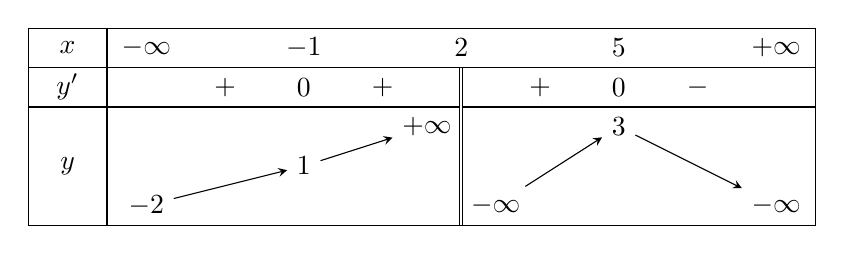
\begin{tikzpicture}[yscale=.5,xscale=1,
            kxd/.pic={\draw[double] (90:.5)--(-90:.5);}]
            \begin{scope}[shift={(-.5,.5)}]
                \draw
                (0,0) rectangle +(10,-5)
                (0,-1)--+(0:10) (0,-2)--+(0:10) (1,0)--+(-90:5);
            \end{scope}
            \path
            (0,0) node{$x$} % <<< dòng 1
            ++(0:1) node{$-\infty$}
            ++(0:2) node{$-1$}
            ++(0:2) node{$2$}
            ++(0:2) node{$5$}
            ++(0:2) node{$+\infty$}
            (0,-1) node{$y'$} % <<< dòng 2
            ++(0:2) node{$+$}
            ++(0:1) node{$0$}
            ++(0:1) node{$+$}
            ++(0:1) pic[scale=.5]{kxd}
            ++(0:1) node{$+$}
            ++(0:1) node{$0$}
            ++(0:1) node{$-$}
            (0,-3) node{$y$} % <<< dòng 3
            ++(0:1)+(-90:1) node (A) {$-2$}
            ++(0:2) node (B) {$1$}
            ++(0:2)+(90:1) node[left] (F) {$+\infty$}
            ++(0:0) pic[scale=1.5]{kxd}
            ++(0:0)+(-90:1) node[right] (C) {$-\infty$}
            ++(0:2)+(90:1) node(D) {$3$}
            ++(0:2)+(-90:1) node(E) {$-\infty$};
            \begin{scope}[-stealth]
                \draw (A)--(B);
                \draw (C)--(D);
                \draw (D)--(E);
                \draw (B)--(F);
            \end{scope}
        \end{tikzpicture}
    \end{center}
    Hàm số đã cho có bao nhiêu cực trị?
    \choice
    {$2$}{\True $1$}{$3$}{$4$}
    \loigiai{
        Dựa vào bảng biến thiên, hàm số có duy nhất một điểm cực trị.}
\end{ex}

%%==========Câu 48
\begin{ex}%[2D1B2-2]
    Cho hàm số $y=f(x)$ liên tục trên $[a;b]$ và có đồ thị như hình vẽ bên. Số điểm cực đại của hàm số đã cho là
    \begin{center}
        \begin{tikzpicture}[>=stealth,line join=round, line cap=round, font=\footnotesize,scale=0.8]
            \draw[-stealth](-4,0)--(0,0)node[below left]{$O$}--(4,0)node[below left]{$x$};
            \draw[-stealth](0,-2)--(0,3)node[below left]{$y$};
            \draw[dashed]
            (-3,0)node[above]{$a$}--(-3,-1)
            (3,0)node[below]{$b$}--(3,2)
            ;
            \draw[smooth,thick,blue]
            (-3,-1)..controls+(85:2) and+(180:.5)..(-2,2)
            ..controls+(0:.5) and+(180:.5)..(-.75,0.5)
            ..controls+(0:.5)and+(180:.5)..(1,2.5)
            ..controls+(0:.5)and+(180:.25)..(2,.75)
            ..controls+(0:.5)and+(65:.3)..(3,2)
            %..controls+(0:.5)and+(110:.3)..(3,-1.5)
            ;
        \end{tikzpicture}
    \end{center}
    \choice
    {$4$}
    {$1$}
    {\True $2$}
    {$3$}
    \loigiai{
        Dựa vào đồ thị hàm số đã cho có $2$ điểm cực đại.
    }
\end{ex}

%\textbf{THIẾU TRANG 59-65}
\begin{ex}%[2D1K2-2]
    \immini
    {
        Cho hàm số $y=f(x)$ xác định, liên tục trên đoạn $[-2;2]$ và có đồ thị là đường cong trong hình vẽ bên. Đường thẳng đi qua hai điểm cực trị của đồ thị hàm số đã cho có phương trình
        \choice
        {$y=-\dfrac{1}{2}x+1$}
        {$y=-\dfrac{1}{2}x$}
        {$y=-2x+1$}
        {\True $y=-2x$}
    }
    {
        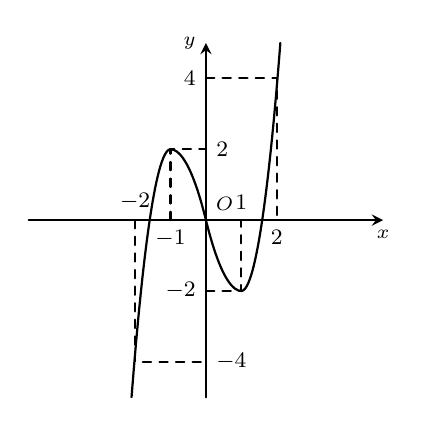
\begin{tikzpicture}[line join = round, line cap = round,>=stealth,thick,font=\footnotesize,scale=0.45]
            \def\a{1} % Hệ số a phải khác 0
            \def\b{0}
            \def\c{-3}
            \def\d{0}
            %\draw[color=gray,dash pattern=on 1pt off 1pt,xstep=1.0cm,ystep=1.0cm] (-5.2,-5.2) grid (5.2,5.2);
            \draw[->] (-5,0) -- (5,0)node[below]{\scriptsize $x$};
            \draw[->] (0,-5) -- (0,5) node[left] {\scriptsize $y$};
            \draw[dashed] (0,0)node[above right=-.1]{\scriptsize $O$} (-2,0)node[above]{$-2$}|-(0,-4)node[right]{$-4$} (-1,0)node[below]{$-1$}|-(0,2)node[right]{$2$} (0,-2)node[left]{$-2$}-|(1,0)node[above]{$1$} (0,4)node[left]{$4$}-|(2,0)node[below]{$2$};
            \clip (-5,-5)rectangle(5,5);
            %\draw[thick,samples=150,smooth,domain=-5:5] plot(\x,{\a*(\x)^3+(\b)*(\x)^2+(\c)*\x+(\d)});
            \draw (-2.1,-5) parabola bend (-1,2) (0,0) parabola bend (1,-2) (2.1,5);
        \end{tikzpicture}
    }
    \loigiai{
        Dựa vào đồ thị ta thấy Đồ thị hàm số có hai điểm cực trị là $A(-1;2)$ và $B(1,-2)$, phương trình đường thẳng qua hai điểm cực trị là
        \[\dfrac{x+1}{-1-1}=\dfrac{y-2}{2+2}\Leftrightarrow y=-2x.\]
    }
\end{ex}
\begin{ex}%[2D1B2-2]
    Cho hàm số $y=f(x)$ có bảng biến thiên như hình vẽ.
    \begin{center}
        
\begin{tikzpicture}
            \tkzTabInit[espcl=2.5,lgt=1]
            {$x$/0.6,$y'$/0.6,$y$/2.2}
            {$-\infty$,$ -1 $,$ 2 $,$5$,$+\infty$}
            \tkzTabLine{,-,0,+,d,-,0,-,}
            \tkzTabVar{+/$+\infty$,-/$ -1 $,+/$ 3 $,R/,-/$-\infty$}
            \tkzTabVal{3}{5}{0.5}{}{$1$}
        \end{tikzpicture}
    \end{center}
    Khoảng cách giữa hai điểm cực trị của đồ thị hàm số đã cho bằng
    \choice
    {$\sqrt{5}$}
    {$2 \sqrt{10}$}
    {$\sqrt{13}$}
    {\True $ 5 $}
    \loigiai{
        Điểm cực tiểu của đồ thị hàm số là $ (-1;-1) $, điểm cực đại của đồ thị hàm số là $ (2;3) $. Khi đó khoảng cách hai điểm cực trị là \[ \sqrt{(-1-2)^2+(-1-3)^2}=5. \]
    }
\end{ex}
\begin{ex}%[2D1B2-2]
    Cho hàm số $y=f(x)$ liên tục trên $\mathbb{R}$ và có bảng biến thiên như hình vẽ.
    \begin{center}
        
\begin{tikzpicture}
            \tkzTabInit[espcl=2.5,lgt=1]
            {$x$/0.6,$y'$/0.6,$y$/2.0}
            {$-\infty$,$ -4$,$ -2 $,$ 0 $,$+\infty$}
            \tkzTabLine{,+,0,-,d,-,0,+,}
            \tkzTabVar{-/$-\infty$,+/$ -1$,-D+/$-\infty$/$+\infty$,-/$ 3 $,+/$+\infty$}
        \end{tikzpicture}
    \end{center}
    Đường thẳng đi qua hai điểm cực trị của đồ thị hàm số đã cho có phương trình
    \choice
    {$y=x-3$}
    {\True $y=x+3$}
    {$y=-x+3$}
    {$y=-x-3$}
    \loigiai{
        Hai điểm cực trị của đồ thị hàm số là $ (-4;-1) $ và $ (0;3) $. Đường thẳng qua hai điểm cực trị có dạng $ y=ax+b $ nên \[ \heva{&-1=a \cdot (-4)+b\\&3=a \cdot 0+1} \Leftrightarrow\heva{&a=1\\&b=3} \Rightarrow y=x+3. \]
    }
\end{ex}
\begin{ex}%[2D1B2-2]
    Cho hàm số $ y=f(x) $ có $ f'(x)=x(x+2)^2(x-1)^4(x-2)^3 $. Hàm số đã cho đạt cực đại tại
    \choice
    {$ x=-2 $}
    {$ x=1 $}
    {\True $ x=0 $}
    {$ x=2 $}
    \loigiai{
        Ta có $ f'(x)=0 \Leftrightarrow \hoac{& x=0\\&x=-2\\&x=1\\&x=2.} $\\
        Bảng biến thiên.
        \begin{center}
            
\begin{tikzpicture}
                \tkzTabInit[espcl=2.5,lgt=1.5]
                {$x$/0.7,$y'$/0.7,$y$/2}
                {$-\infty$,$-2$,$0$,$1$,$ 2 $,$+\infty$}
                \tkzTabLine{,+,z,+,z,-,z,-,z,+,}
                \tkzTabVar{-/,R/,+/,R/,-/,+/}
            \end{tikzpicture}
        \end{center}
        Từ bảng biến thiên ta được hàm số đạt cực đại tại $ x=0 $.
    }
\end{ex}
\begin{ex}%[2D1B2-4]
    Tìm tất cả các giá trị của tham số $m$ để hàm số $y=x^3-3x^2+mx+1$ có hai điểm cực trị.
    \choice
    {$m\le3$}
    {$m>3$}
    {$m>-3$}
    {\True $m<3$}
    \loigiai{
        Ta có $y'=3x^2-6x+m$.\\
        Hàm số có hai điểm cực trị $\Leftrightarrow $ phương trình $y'=0$ có hai nghiệm phân biệt\\
        $$\Leftrightarrow \Delta'=9-3m>0 \Leftrightarrow m<3.$$
    }
\end{ex}
\begin{ex}%[2D1B2-5]
    Tìm $m$ để hàm số $y=mx^4-m^3x^2+2018$ có ba điểm cực trị.
    \choice
    {$ m>0 $}
    {$ m\in \mathbb{R}\setminus \left\lbrace 0 \right\rbrace  $}
    {\True $ m\ne 0 $}
    {Không tồn tại $m$}
    \loigiai{
        Tập xác định $\mathscr{D}=\mathbb{R}$.\\
        Ta có $y'=4mx^3-2m^3x$.\\
        \begin{enumerate}[.]
            \item Nếu $m=0$ thì $y'=0,\quad \forall x\in \mathbb{R}$. Suy ra hàm số không có cực trị. Vậy $m=0$ loại.
            \item Xét $m\ne0$\\
            $y'=0\Leftrightarrow\hoac{&x=0\\&2x^2-m^2=0.}$\\
            Hàm số có ba điểm cực trị khi và chỉ khi $y'=0$ có ba nghiệm phân biệt $\Leftrightarrow m\ne 0$.
        \end{enumerate}
        Vậy $m\ne0$ là giá trị cần tìm.
    }
\end{ex}
\begin{ex}%[2D1B2-1]
    Hàm số nào sau đây đạt cực đại tại $x=1$?
    \choice
    {\True $y=2\sqrt{x}-x$}
    {$y=x^5-5x^2+5x-13$}
    {$y=x^4-4x+3$}
    {$y=x+\dfrac{1}{x}$}
    \loigiai{
        Hàm số $y=2\sqrt{x}-x$ có tập xác định $\mathscr{D}=[0;+\infty)$, liên tục và có đạo hàm trên $(0;+\infty)$.\\
        Ta có $y'=\dfrac{1}{\sqrt{x}}-1=0\Leftrightarrow x=1$ và $y''=-\dfrac{1}{2x\sqrt{x}}\Rightarrow y''(1)<0$. Do đó $x_{\textrm{CĐ}}=1$.
    }
\end{ex}
\begin{ex}%[2D1B2-3]
    Tìm tất cả các giá trị của tham số $m$ để hàm số $y=x^3 -2mx^2 +m^2 x+1$ đạt cực tiểu tại $x=1$.
    \choice
    {$m=1,m=3$}
    {\True $m=1$}
    {$m=3$}
    {Không tồn tại $m$}
    \loigiai{
        Ta có $y'=3x^2-4mx+m^2$, $y''=6x-4m$.\\
        Hàm số đạt cực tiểu tại $x=1$ khi và chỉ khi
        $$\heva{& y'(1) = 0 \\ & y''(1) >0 } \Leftrightarrow \heva{ & m^2-4m+3 = 0 \\ & 6-4m > 0 } \Leftrightarrow \heva{ & \hoac {& m=1 \\ & m = 3} \\ & m < \dfrac{3}{2}} \Leftrightarrow m = 1.$$
    }
\end{ex}
\begin{ex}%[2D1B2-3]
    Hàm số $y=x^3+2ax^2+4bx-2018$ $(a,b\in\mathbb{R})$ đạt cực trị tại $x=-1$. Khi đó hiệu $a-b$ là
    \choice
    {$-1$}
    {$\dfrac{4}{3}$}
    {\True $\dfrac{3}{4}$}
    {$-\dfrac{3}{4}$}
    \loigiai{
        Ta có $y'=3x^2+4ax+4b$.\\
        Hàm số đạt cực trị tại $x=-1$ nên $y'(-1)=0\Rightarrow 3-4a+4b=0\Rightarrow a-b=\dfrac{3}{4}$.}
\end{ex}
\begin{ex}%[2D1K2-4]
    Tính tổng các giá trị của tham số $m$ sao cho   hàm số $y=  x^3  - 3 x^2 + m^2 -2m $ có  giá trị cực đại bằng $3$?
    \choice
    {\True $2$}
    {$-2$}
    {$3$}
    {$-3$}
    \loigiai{
        Tập xác định $\mathscr{D} = \mathbb{R}$.\\
        $y'=3x^2 - 6x =0\Leftrightarrow \hoac{&x=0\\ &x=2.}$\\
        Ta có $y''=6x - 6$.\\
        Tại $x_1=0$, $y'(x_1) = 0$, $y''(x_1) =  -6<0$, suy ra điểm $M_1(0;y(0)= m^2-2m)$ là điểm    cực đại của đồ thị hàm số.\\
        Tại $x_2=2$, $y'(x_2) = 0$, $y''(x_2) =   6>0$, suy ra điểm $M_2(2;y(-2)=m^2 - 2m -4)$ là điểm    cực tiểu của đồ thị hàm số.\\
        Hàm số $y=  x^3  - 3 x^2 + m^2 -2m $ có  giá trị cực đại bằng $3$
        \[\Leftrightarrow y(0) = 3 \Leftrightarrow m^2-2m = 3 \Leftrightarrow \hoac{&m=-1 \\ &m=3.}\]
        Vậy tổng các giá trị $m$ thỏa mãn yêu cầu bài toán là $-1+ 3 = 2$.
    }
\end{ex}
\begin{ex}%[2D1K2-5]
    Biết đồ thị hàm số $ y = x^4 -2mx^2 +1$ có ba điểm cực trị $ A(0;1) $, $ B
    $, $ C $ sao cho trung điểm $ I $ của $ BC $ thuộc đường thẳng $ d \colon
    y+1=0 $. Khi đó $ m $ thuộc tập nào sau đây?
    \choice
    {$\{-4;0;4\} $}
    {\True $\{-\sqrt{2};0;\sqrt{2}\} $}
    {$\{-1;0;1\} $}
    {$\{-2;0;2\} $}
    \loigiai{
        Ta có $ y' = 4x^3 - 4mx  $, $ y' =0 \Leftrightarrow 4x^3 - 4mx = 0
        \Leftrightarrow \hoac{& x=0 \\ & x^2=m.} $\\
        Để hàm số có ba cực trị thì $ m > 0 $. \hfill $ (*) $\\
        Giả sử đồ thị hàm số có ba điểm cực trị là $ A(0;1) $, $ B(-\sqrt{m};
        1-m^2) $, $	C(\sqrt{m}; 1-m^2) $.\\
        Tọa độ trung điểm $ I $ của $ BC $ là $ I(0;1-m^2) $.
        $$ I \in d \Leftrightarrow 1-m^2+1 = 0 \Leftrightarrow m = \pm \sqrt{2}
        .	$$
        Kết hợp với $ (*) $ suy ra $ m = \sqrt{2} $.
    }
\end{ex}
\begin{ex}%[2D1K2-4]
    Biết $ m_0 $ là giá trị của tham số $ m $ để hàm số $ y = x^3-3x^2+mx-1 $
    có hai điểm cực trị $ x_1 $, $ x_2 $ sao cho $ x_1^2+x_2^2-x_1x_2=13 $.
    Mệnh đề nào sau đây đúng?
    \choice
    {$ m_0 \in (-1;7) $}
    {$ m_0 \in (7;10) $}
    {\True $ m_0 \in (-15;-7) $}
    {$ m_0 \in (-7;-1) $}
    \loigiai{
        Ta có $ y' = 3x^2-6x+m$.  \\
        Để hàm số có hai cực trị thì phương trình $ y'=0 $ có $ 2 $ nghiệm phân
        biệt \[ \Leftrightarrow \Delta' > 0 \Leftrightarrow 9-3m > 0
        \Leftrightarrow m <3. \tag{$ * $}\]
        Gọi $ x_1 $, $ x_2 $ là hai điểm cực trị của hàm số. Suy
        ra $ \heva{& S = x_1+x_2 = 2 \\ & P = x_1x_2 = \dfrac{m}{3}.} $ \\
        Khi	đó
        \begin{eqnarray*}
            x_1^2+x_2^2-x_1x_2=13 &\Leftrightarrow& (x_1+x_2)^2-3x_1x_2=13 \\
            &\Leftrightarrow& S^2 - 3P=13 \\
            &\Leftrightarrow& 4 - 3 \cdot \dfrac{m}{3} =13 \\
            &\Leftrightarrow& m = -9.
        \end{eqnarray*}
        Kết hợp với $ (*) $ suy ra $ m_0 = -9 \in (-15;-7) $.
    }
\end{ex}
\begin{ex}%[2D1K2-4]
    Có bao nhiêu số thực $m$ để đồ thị hàm số $y=x^{3}-3x^{2}+m$ có hai điểm cực trị $A$ và $B$ sao cho tam giác $OAB$ vuông tại $O$?
    \choice
    {\True$2$}
    {$1$}
    {$3$}
    {$0$}
    \loigiai{
        Tập xác định: $\mathscr{D}=\mathbb{R}$.\\
        Ta có  $y'=3x^{2}-6x$.\\
        $y'=3x^{2}-6x=0
        \Leftrightarrow \hoac{& x=2 \Rightarrow y=m-4 \\& x=0 \Rightarrow y=m}$\\
        Vậy hàm số có 2 điểm cực trị $A(0;m);B(2;m-4)$.\\
        Ta có $\vec{OA}=(0;m);\vec{OB}=(2;m-4)$.\\
        Để tam giác $OAB$ vuông tại $O$ thì $m \neq 0$ và $\vec{OA} \cdot \vec{OB}=0 \Leftrightarrow  m \cdot (m-4)=0
        \Leftrightarrow \hoac{& m=0 \quad \text{(loại)} \\ &m=4.}$\\
        Vậy có $1$ giá trị của $m$.
    }
\end{ex}
\begin{ex}%[2D1B2-7]
    Tập hợp tất cả các giá trị thực của tham số $ m $ để hàm số $ y=x^4+(m^2-2)x^2+2 $ có một điểm cực trị là
    \choice
    {\True $\left(-\infty;-\sqrt{2} \right] \cup \left[\sqrt{2};+\infty \right)$}
    {$\left(-\sqrt{2} ;\sqrt{2}\right) $}
    {$\left[-\sqrt{2} ;\sqrt{2}\right] $}
    {$\left(-\infty;-\sqrt{2} \right) \cup \left(\sqrt{2};+\infty \right) $}
    \loigiai{
        Hàm trùng phương có 1 điểm cực trị $ \Leftrightarrow ab \ge 0 \Leftrightarrow m^2-2 \ge 0 \Leftrightarrow m \le -\sqrt{2} $ hoặc $ m \ge \sqrt{2} $.
    }
\end{ex}
\begin{ex}%[2D1K2-5]
    Có bao nhiêu giá trị nguyên của $m\in (-5;5)$ sao cho hàm số $y= m^2 x^4 + (m - 4)x^2 + m$ có $2$ điểm cực tiểu và $1$ điểm cực đại?
    \choice
    {$6$}
    {$8$}
    {\True $7$}
    {$5$}
    \loigiai{
        Tập xác định $\mathscr{D}=\mathbb{R}$.\\
        $y’=  4m^2 x^3 + 2(m-4)x=0\Leftrightarrow \hoac{&x = 0 \\ & 4m^2 x^2 +2(m-4)=0.}$\\
        Hàm số có $2$ điểm cực tiểu và $1$ điểm cực đại thì bảng biến thiên có dạng
        \begin{center}
            \begin{tikzpicture}
                \tkzTabInit[lgt=1,espcl=2.5]%
                {$x$/1,%
                    $y'$ /1,%
                    $y$/2}%
                {$-\infty$ , $x_1$,0, $x_2$ , $+\infty$}%
                \tkzTabLine{ ,-, 0,+,0,-, 0 ,+, }
                %\tkzTabSlope{1//+\infty,3/-1 /+1}
                \tkzTabVar %
                {+ / $+\infty$ ,
                    - / $y_{\text{CT}}$ ,
                    + / $y_{\text{CĐ}}$ ,
                    - / $y_{\text{CT}}$ ,
                    + / $+\infty$ }
            \end{tikzpicture}
        \end{center}
        Từ bảng biến thiên suy ra, để hàm số có $2$ điểm cực tiểu và $1$ điểm cực đại, phương trình $4m^2 x^2 +2(m-4)=0$ có hai nghiệm phân biệt khác $0$
        \[\Leftrightarrow \heva{&m^2\neq 0\\ &-\dfrac{2(m-4)}{4m^2}>0}  \Leftrightarrow m<0 \vee 0<m<4.\]
        Vì $m\in \mathbb{Z}$ và $m\in (-5;5)$   nên $m\in \{-4;-3;-2;-1;1;2;3\}$. Vậy có $7$ giá trị $m$ thỏa mãn yêu cầu bài toán.
    }
\end{ex}
\begin{ex}%[2D1K2-2]
    \immini{Cho hàm số $y=f(x)$ có đạo hàm liên tục trên $\mathbb{R}$ và có đồ thị hàm số $f\left(3-x\right)$ như hình vẽ bên. Hỏi hàm số $y=f\left(x^2-2x\right)$ có mấy cực trị?
        \choice
        {\True $1$}
        {$2$}
        {$3$}
        {$4$}
    }
    {\begin{tikzpicture}[scale=.6,>=stealth, font=\footnotesize, line join=round, line cap=round]
            \def\xmin{-5} \def\xmax{5}
            \def\ymin{-5} \def\ymax{5}
            %\draw[color=gray!50,dashed] (\xmin,\ymin) grid (\xmax,\ymax);
            \draw[->] (\xmin,0)--(\xmax,0) node [below]{$x$};
            \draw[->] (0,\ymin)--(0,\ymax) node [left]{$y$};
            \node at (0,0) [below left]{$O$};
            \draw[dashed] (-3,0)--(-3,-3)--(0,-3);
            \draw[dashed] (3,0)--(3,3)--(0,3);
            \draw[dashed] (-1,0)--(-1,1)--(0,1);
            \draw[dashed] (1,0)--(1,-1)--(0,-1);
            \clip (\xmin+0.1,\ymin+0.1) rectangle (\xmax-0.5,\ymax-0.1);
            \draw[smooth,samples=300][domain=-4:0] plot(\x,{-(\x)^2-2*(\x)});
            \draw[smooth,samples=300][domain=0:4] plot(\x,{(\x)^2-2*(\x)});
            \foreach \x in {-4,-3,-2,-1,1,2,3,4}
            \draw[thin] (\x,1pt)--(\x,-1pt) node [below] {$\x$};
            \foreach \y in {-4,-3,-2,-1,1,2,3,4}
            \draw[thin] (1pt,\y)--(-1pt,\y) node [left] {$\y$};
    \end{tikzpicture}}
    \loigiai{
        Ta có $y'=\left(f(3-x)\right)'=-f'(3-x)$.\\
        Chọn $f'(3-x)=(x+1)(x-1)\Rightarrow-f'(3-x)=-(x+1)(x-1)$.\\
        Đặt $t=3-x$ ta có $x=3-t$\\
        Vậy $f'(t)=-(4-t)(2-t)\Rightarrow f'(x)=-(4-x)(2-x)\quad(*)$\\
        Ta có $y=f(x^2-2x)\Rightarrow y'=2(x-1)f'(x^2-2x)$\\
        Từ (*) ta có
        $y'=2(x-1)f'(x^2-2x)=2(x-1)(4-x^2+2x)(2-x^2+2x)$.\\
        Nhận thấy với $y'=0\Leftrightarrow x=1$ như vậy $y'$ chỉ đổi dấu $1$ lần qua $x=1$.\\ Vậy hàm số $y=f\left(x^2-2x\right)$ có một cực trị.
    }
\end{ex}
\begin{ex}%[2D1K2-2]
    \immini
    {
        Cho hàm số $y=f(x)$ liên tục trên $\mathbb{R}$, có đồ thị hàm số $y=f'\left(x^2+2x\right)$ như hình vẽ. Tìm số điểm cực trị của hàm số $g(x)=f(2x-x^2)$.
        \choice
        {$2$}
        {$4$}
        {\True $3$}
        {$5$}
    }
    {
        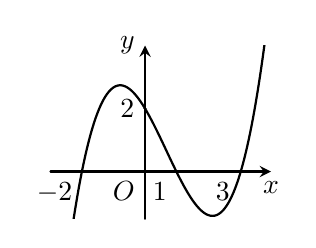
\begin{tikzpicture}[line join=round, line cap=round,>=stealth,thick,scale=.4]
            \tikzset{label style/.style={font=\footnotesize}}
            \def \xmin{-3}
            \def \xmax{4}
            \def \ymin{-1.5}
            \def \ymax{4}
            \def \hamso{.33*(\x)^3-.67*(\x)^2-1.67*\x+2}
            \draw[->] (\xmin,0)--(\xmax,0) node[below] {$x$};
            \draw[->] (0,\ymin)--(0,\ymax) node[left] {$y$};
            \draw (0,0) node [below left] {$O$};
            \foreach \x in {-2,1,3}
            \draw[thin] (\x,1pt)--(\x,-1pt) node [below left] {$\x$};
            \foreach \y in {2}
            \draw[thin] (1pt,\y)--(-1pt,\y) node [left] {$\y$};
            \begin{scope}
                \clip (\xmin+0.01,\ymin+0.01) rectangle (\xmax-0.01,\ymax-0.01);
                \draw[samples=200,domain=\xmin+0.01:\xmax-0.01,smooth,variable=\x] plot (\x,{\hamso});
            \end{scope}
        \end{tikzpicture}
    }
    \loigiai{
        Ta có $f'\left(x^2+2x\right)=0\Leftrightarrow\hoac{&x=-2\\&x=1\\&x=3}\Rightarrow f'(x)=0\Leftrightarrow\hoac{&x=0\\&x=3\\&x=15.}$\\
        Xét: $g'(x)=(2-2x)\cdot f'\left(2x-x^2\right)$.\\
        Ta có $g'(x)=0\Leftrightarrow\hoac{&x=1\\&2x-x^2=0\\&2x-x^2=3\\&2x-x^2=15}\Leftrightarrow\hoac{&x=1\\&x=0\\&x=2.}$\\
        Thấy rằng $g'(x)=0$ có 3 nghiệm đơn nên hàm số $y=g(x)$ có 3 điểm cực trị.
    }
\end{ex}
\begin{ex}%[2D1G2-2]
    Cho hàm số $f(x)$ có bảng biến thiên của hàm
    số $f'(x)$ bên dưới.
    \begin{center}
        \begin{tikzpicture}
            \tkzTabInit[nocadre=false, lgt=1.2,espcl=2.5,deltacl=0.6]
            {$x$/0.6, $f'(x)$ /3}
            {$-\infty$,$-1$,$0$,$1$,$+\infty$}
            \path
            (N11)node[below=0.1cm,fill=white](A){$+\infty$}
            (N22)node[above=0.1cm,fill=white](B){$-3$}
            (barycentric cs:N31=2,N32=1)node[fill=white](C){$2$}
            (barycentric cs:N41=1,N42=2)node[fill=white](D){$-1$}
            (N51)node[below=0.1cm,fill=white](E){$+\infty$}
            ;
            \draw[-stealth](A)--(B);
            \draw[-stealth](B)--(C);
            \draw[-stealth] (C)--(D);
            \draw[-stealth] (D)--(E);
        \end{tikzpicture}
    \end{center}
    Số điểm cực trị của hàm số $y=f (x^2-2x)$ là
    \choice
    {$9$}
    {$3$}
    {\True $7$}
    {$5$}
    \loigiai{
        \immini{
            Ta có $y'=(2x-2)f'(x^2-2x)$.\\
            $y'=0\Leftrightarrow \hoac{&x=1\\&x^2-2x=a&(a<-1)\\&x^2-2x=b&(-1<b<0)\\&x^2-2x=c&(0<c<1)\\&x^2-2x=d&(d>1).}$}
        {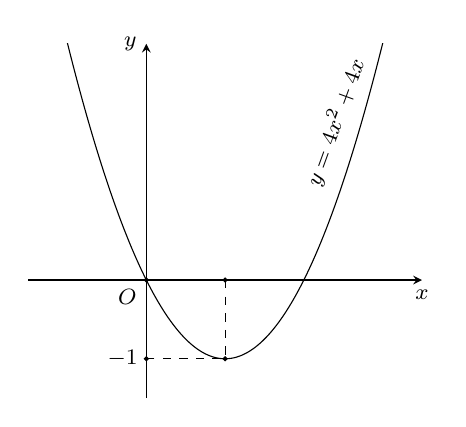
\begin{tikzpicture}[scale=1,>=stealth,font=\footnotesize]
                \def\mx{-1.5} \def\max{3.5}
                \def\my{-1.5} \def\may{3}
                \def\hamso(#1,#2){plot [samples=200,smooth,domain=#1:#2](\x,{
                        (\x)^2-2*(\x)
                    })}
                \draw[fill=black] (0,-1)circle (.7pt) node[shift={(180:.3)}]{$-1$}
                (0,0)circle (.7pt) node [below left] {$O$}
                (1,-1)circle (.7pt) (1,0)circle (.7pt)
                ;
                \draw[dashed,thin] (1,0)|-(0,-1);
                %===========================================
                \draw[->] (\mx,0)--(\max,0) node[below] {$x$};
                \draw[->] (0,\my)--(0,\may) node[left] {$y$};
                \clip (\mx,\my) rectangle (\max,\may);
                \draw \hamso(\mx,\max)(2.4,2)node[rotate=70]{$y=4x^2+4x$};
        \end{tikzpicture}}
        \noindent
        Dựa vào bảng biến thiên của hàm số $g(x)=x^2-2x$ ta có phương trình $y'=0$ có $7$ nghiệm đơn phân biệt.\\
        Suy ra số điểm cực trị của hàm số $y=f (x^2-2x)$ là $7$.
    }
\end{ex}
\begin{ex}%[2D1G2-2]
    \immini{
        Cho hàm số $f(x)=ax^4+bx^3+cx^2+dx+e$ ($ae<0$). Đồ thị hàm số $y=f'(x)$ như hình bên. Hỏi hàm số $y=\left|4f(x)-x^2\right|$ có bao nhiêu điểm cực tiểu?
        \choice
        {$2$}
        {\True $3$}
        {$5$}
        {$4$}
    }{
        \begin{tikzpicture}[scale=.8, font=\footnotesize, line join=round, line cap=round, >=stealth]
            \draw[->] (-2,0)--(3,0) node[above] {$x$};
            \draw[->] (0,-1)--(0,3) node[right] {$y$};
            \draw[fill=black] (0,0) circle (1pt) node[above left] {$O$};
            \draw[fill=black] (2,0) circle (1pt) node[below]{$2$};
            \draw[fill=black] (-1,0) circle (1pt) node[above]{$-1$};
            \draw[fill=black] (0,1) circle (1pt) node[left]{$1$};
            \draw[fill=black] (0,-0.5) circle (1pt) node[right]{$-\dfrac{1}{2}$};
            \begin{scope}
                \clip (-2,-1) rectangle (3,3);
                \draw[samples=200,domain=-2:3,smooth] plot (\x,{-0.93*(\x)^3+0.93*(\x)^2+2.37*(\x)});
            \end{scope}
            \draw[fill=black,dashed] (-1,0)--(-1,-0.5)circle (1pt)--(0,-0.5)
            (0,1)--(2,1)circle (1pt)--(2,0);
        \end{tikzpicture}
    }
    \loigiai{
        Hàm số $y=f(x)$ xác định trên $\mathbb{R}$ và $f'(x)=4ax^3+3bx^2+2cx+d$.\\
        Dựa vào đồ thị hàm số $y=f'(x)$ ta thấy $4a<0\Leftrightarrow a<0$. \\
        Ta có $ae<0$ mà $a<0$ nên suy ra $e>0$. \\
        Xét hàm số $g(x)=4f(x)-x^2$ ta có $g'(x)=4f'(x)-2x=4\left[f'(x)-\dfrac{x}{2}\right]$.
        \immini{
            Ta thể hiện đường thẳng $y=\dfrac{x}{2}$ cùng với đồ thị hàm số $y=f'(x)$ lên cùng một hệ trục tọa độ như hình bên.\\
            Dựa vào đồ thị ta thấy $g'(x)=0\Leftrightarrow \hoac{&x=-1\\&x=0\\&x=2.}$\\
            Bảng biến thiên
        }{
            \begin{tikzpicture}[scale=1, font=\footnotesize, line join=round, line cap=round, >=stealth]
                \draw[->] (-2,0)--(3,0) node[above] {$x$};
                \draw[->] (0,-1)--(0,3) node[right] {$y$};
                \draw[fill=black] (0,0) circle (1pt) node[above left] {$O$};
                \draw[fill=black] (2,0) circle (1pt) node[below]{$2$};
                \draw[fill=black] (-1,0) circle (1pt) node[above]{$-1$};
                \draw[fill=black] (0,1) circle (1pt) node[left]{$1$};
                \draw[fill=black] (0,-0.5) circle (1pt) node[right]{$-\dfrac{1}{2}$};
                \begin{scope}
                    \clip (-2,-1) rectangle (3,3);
                    \draw[samples=200,domain=-2:3,smooth] plot (\x,{-0.93*(\x)^3+0.93*(\x)^2+2.37*(\x)});
                    \draw[smooth] plot (\x,{0.5*(\x)});
                \end{scope}
                \draw[fill=black,dashed] (-1,0)--(-1,-0.5)circle (1pt)--(0,-0.5)
                (0,1)--(2,1)circle (1pt)--(2,0);
            \end{tikzpicture}
        }
        \begin{center}
            \begin{tikzpicture}[scale=1, font=\footnotesize, line join=round, line cap=round, >=stealth]
                \tkzTabInit[nocadre=false,lgt=1.2,espcl=2.5,deltacl=0.6]
                {$x$/0.6,$g'(x)$/0.6,$g(x)$/3}
                {$-\infty$,$x_1$,$-1$,$0$,$2$,$x_2$,$+\infty$}
                \tkzTabLine{,,+,,0,-,0,+,0,,-,,}
                \tkzTabVar{-/$-\infty$,R,+/$g(-1)$,R,R,R,R}
                \node[fill=white] at ($(N22)!0.5!(N23)$) (0){$0$}
                (N32)node[below](1){\phantom{$g(-1)$}}
                ($(N42)!0.35!(N43)$)node[fill=white](2){$4e$}
                (N52)node[below](3){$g(2)$}
                ($(N62)!0.5!(N63)$)node[fill=white](4){$0$}
                (N73)node[above](5){$-\infty$};
                \draw[->] (1)--(2);
                \draw[->] (2)--(3);
                \draw (3)--(4);
                \draw[->] (4)--(5);
                \draw[dashed] ($(N12)!0.5!(N13)$)--($(N72)!0.5!(N73)$);
            \end{tikzpicture}
        \end{center}
        Từ đó ta có bảng biến thiên của hàm số $y=|g(x)|$ như sau
        \begin{center}
            \begin{tikzpicture}[scale=1, font=\footnotesize, line join=round, line cap=round, >=stealth]
                \tkzTabInit[nocadre=false,lgt=1.2,espcl=2.5,deltacl=0.6]
                {$x$/0.6,$|g(x)|$/3}
                {$-\infty$,$x_1$,$-1$,$0$,$2$,$x_2$,$+\infty$}
                \tkzTabVar{+/$+\infty$,-/$0$,+/$g(-1)$,R,R,R,R}
                \node[below] at (N31)(1){\phantom{$g(-1)$}}
                ($(N41)!0.5!(N42)$)node[below](2){$4e$}
                (N51)node[below](3){$g(2)$}
                (N62)node[above](4){$0$}
                (N71)node[below](5){$+\infty$};
                \draw[->] (1)--(2);
                \draw[->] (2)--(3);
                \draw[->] (3)--(4);
                \draw[->] (4)--(5);
            \end{tikzpicture}
        \end{center}
        Dựa vào bảng biến thiên ta suy ra hàm số $y=|g(x)|=\left|4f(x)-x^2\right|$ có $3$ điểm cực tiểu.
    }
\end{ex}
\begin{ex}%[2D1G2-2]
    \immini{Cho hàm số $y=f(x)$ có đạo hàm liên tục trên $\mathbb{R}$ và $f(0)=0$; $f(4) > 4$. Biết hàm $y=f'(x)$ có đồ thị như hình vẽ bên. Số điểm cực trị của hàm số $g(x)=\left|f\left(x^2\right)-2x\right|$ là
        \choice
        {2}
        {1}
        {4}
        {\True 3}
    }{
        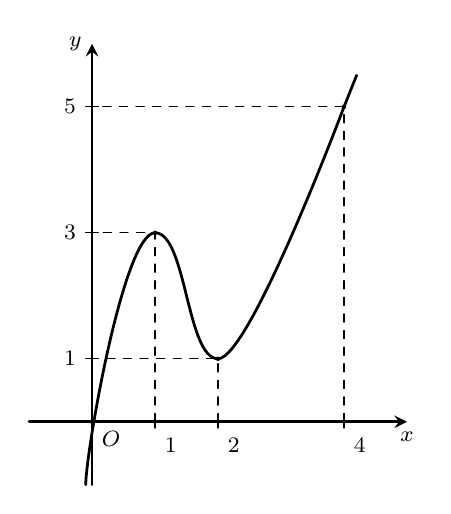
\begin{tikzpicture}[>=stealth,line join=round,line cap=round,font=\footnotesize,scale=0.8]
            \def\xmin{-1} \def\xmax{5}
            \def\ymin{-1} \def\ymax{6}
            \draw[->,line width=1pt] (\xmin,0)--(\xmax,0) node [below]{$x$};
            \draw[->,line width=1pt] (0,\ymin)--(0,\ymax) node [left]{$y$};
            \node at (0,0) [below right]{$O$};
            %\fill (-2,0) node[below left]{$-2$};
            %\fill (1,0) node[below]{$1$};
            \draw[line width=1pt]
            (-0.1,-1)
            .. controls + (90:0.5) and + (180:0.5) .. (1,3)
            .. controls + (0:0.5) and + (180:0.5) .. (2,1)
            .. controls + (0:0.5) and + (180:0) .. (4,5)
            .. controls + (0:0) and + (0:0) .. (4.2,5.5)
            ;
            \foreach \x in {1,2,4}\draw (\x,0.1)--(\x,-0.1) node[below right] {\footnotesize $\x$};
            \foreach \y in {1,3,5}\draw (0.1,\y)--(-0.1,\y) node [left] {\footnotesize $\y$};
            \fill (0.0,0.0) circle (1pt);
            \draw[dashed] (1.0,0)--(1.0,3.0)--(0,3.0);\fill (1.0,3.0) circle (1pt);
            \draw[dashed] (2.0,0)--(2.0,1.0)--(0,1.0);\fill (2.0,1.0) circle (1pt);
            \draw[dashed] (4.0,0)--(4.0,5.0)--(0,5.0);\fill (4.0,5.0) circle (1pt);
        \end{tikzpicture}
    }
    \loigiai{
        Xét $h(x)=f\left(x^2\right)-2x$ $\Rightarrow h'(x)=2x\,f'\left(x^2\right)-2=2\left[x\,f'\left(x^2\right)-1\right]$.\\
        Phương trình: $h'(x)=0\Leftrightarrow x\,f'\left(x^2\right)-1=0. \quad (1)$.\\
        Lập bảng biến thiên của $h(x)$
        \begin{itemize}
            \item Nếu $x< 0 $ thì $x^2>0$, dựa vào đồ thị suy ra $ f'\left(x^2\right)> 0$.
            Phương trình $(1)$ tương đương $f'\left(x^2\right)=\dfrac{1}{x}$ vô nghiệm vì $f'\left(x^2\right)> 0$ và $\forall x<0$.
            \item Nếu $x= 0$ thì
            $(1) \Leftrightarrow 0-1=0$: phương trình vô nghiệm.
            \item Nếu $x > 0$ thì đặt $x^2=t > 0$
            $(1) \Leftrightarrow f'(t)=\dfrac{1}{\sqrt t}$: phương trình có nghiệm duy nhất $t=a\in\left(0\,;1\right)$.
        \end{itemize}
        \begin{center}
            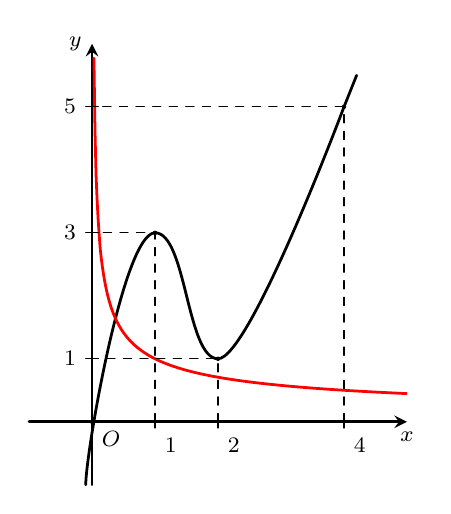
\begin{tikzpicture}[>=stealth,line join=round,line cap=round,font=\footnotesize,scale=0.8]
                \def\xmin{-1} \def\xmax{5}
                \def\ymin{-1} \def\ymax{6}
                \draw[->,line width=1pt] (\xmin,0)--(\xmax,0) node [below]{$x$};
                \draw[->,line width=1pt] (0,\ymin)--(0,\ymax) node [left]{$y$};
                \node at (0,0) [below right]{$O$};
                %\fill (-2,0) node[below left]{$-2$};
                %\fill (1,0) node[below]{$1$};
                \draw[line width=1pt]
                (-0.1,-1)
                .. controls + (90:0.5) and + (180:0.5) .. (1,3)
                .. controls + (0:0.5) and + (180:0.5) .. (2,1)
                .. controls + (0:0.5) and + (180:0) .. (4,5)
                .. controls + (0:0) and + (0:0) .. (4.2,5.5)
                ;
                \clip (\xmin,\ymin) rectangle (\xmax,\ymax);
                \draw[red,line width=1pt,samples=300,domain=0.03:\xmax] plot (\x,{1/((\x)^(1/2))});
                ;
                \foreach \x in {1,2,4}\draw (\x,0.1)--(\x,-0.1) node[below right] {\footnotesize $\x$};
                \foreach \y in {1,3,5}\draw (0.1,\y)--(-0.1,\y) node [left] {\footnotesize $\y$};
                \fill (0.0,0.0) circle (1pt);
                \draw[dashed] (1.0,0)--(1.0,3.0)--(0,3.0);\fill (1.0,3.0) circle (1pt);
                \draw[dashed] (2.0,0)--(2.0,1.0)--(0,1.0);\fill (2.0,1.0) circle (1pt);
                \draw[dashed] (4.0,0)--(4.0,5.0)--(0,5.0);\fill (4.0,5.0) circle (1pt);
            \end{tikzpicture}
        \end{center}
        Vì $h(0)=0$ và $h(2) > 0$ nên ta có bảng biến thiên như sau
        \begin{center}
            \begin{tikzpicture}[scale=1, font=\footnotesize, line join=round, line cap=round, >=stealth]
                \tkzTab
                [lgt=1.5,espcl=3,]
                {$x$/1, $h’(x)$/1, $h(x)$/2, $g(x)$/1.5}
                {$-\infty$, $0$, $\sqrt{a}$,  $2$, $+\infty$}
                {,-, ,-,0,+, ,+,}
                {}
                \tkzTabVar{+/ $ $ ,-/$ $,+/$ $,-/$ $,+/$ $};
                \draw
                (N12)(A)
                (N33)node[above](B){$h(\sqrt{a})$}
                (N52)node[below](C){ }
                ($(N12)!0.5!(N13)$)node[above](D){ }
                ($(N52)!0.5!(N53)$)node[above](E){ }
                (N14)node[above](F){ }
                (N54)node[above](G){ }
                ;
                \foreach \x/\y in {A/B,B/C}
                \draw[-stealth] (\x)--(\y);
                \draw[red,thin] (D)--(E)node[below]{\footnotesize $y=0$};
                \draw[red,thin] (F)--(G)node[above]{\footnotesize $y=0$};
            \end{tikzpicture}
        \end{center}
        Vậy hàm số $g(x)=\left|h(x)\right|$ có 3 cực trị.
    }
\end{ex}

\begin{ex}%[2D1K2-6]
    Cho hàm số $f(x)=x^3-(2m+1)x^2+(3-m)x+2$. Tập hợp tất cả các giá trị thực của tham số $m$ để hàm số $y=f\left(\vert x\vert\right)$ có $3$ cực trị?
    \choice
    {\True $m\ge3$}
    {$-\dfrac{1}{2}<m<3$}
    {$m>3$}
    {$-\dfrac{1}{2}<m\le3$}
    \loigiai{
        Tập xác định $\mathscr{D}=\mathbb{R}$.\\
        Ta có $f\left(|-x|\right)=f\left(|x|\right)$, $\forall x\in\mathbb{R}$ nên $y=f\left(|x|\right)$ là hàm số chẵn.\\
        Do đó, đồ thị hàm số $y=f\left(|x|\right)$ đối xứng qua trục tung.\\
        Suy ra hàm số $y=f\left(|x|\right)$ luôn có một điểm cực trị là $x=0$.\\
        Do đó, hàm số $y=f\left(|x|\right)$ có $3$ cực trị $\Leftrightarrow$ hàm số $y=f(x)$ có $1$ điểm cực trị dương.\\
        \phantom{Do đó, hàm số $y=f\left(|x|\right)$ có $3$ cực trị} $\Leftrightarrow$ phương trình $f'(x)=0$ có $1$ nghiệm dương.\\
        Ta có $f'(x)=3x^2-2(2m+1)x+3-m$, $\Delta'=(2m+1)^2-3(3-m)=4m^2+7m-8$.\\
        \textbf{Trường hợp 1: }\\
        Phương trình $3x^2-2(2m+1)x+3-m=0$ nhận $x=0$ làm nghiệm $\Rightarrow 3-m=0\Leftrightarrow m=3$.\\
        Với $m=3$ ta có $3x^2-14x=0\Leftrightarrow \hoac{&x=0\\&x=\dfrac{14}{3}}$ (thỏa mãn).\\
        \textbf{Trường hợp 2: }\\
        Phương trình $3x^2-2(2m+1)x+3-m=0$ có $2$ nghiệm trái dấu\\
        $\Leftrightarrow 3(3-m)<0\Leftrightarrow m>3$.\\
        Kết hợp hai trường hợp ta có $m\ge3$.
    }
\end{ex}
\Closesolutionfile{ans}
%\indapan{10}{ans/2D1-2-DEON-1}